% Copyright 2013 by Reza Housseini
%
% This file may be distributed and/or modified
%
% 1. under the LaTeX Project Public License and/or
% 2. under the GNU Public License.
%
% See the file LICENSE for more details.

\documentclass[tikz]{standalone}
\begin{document}
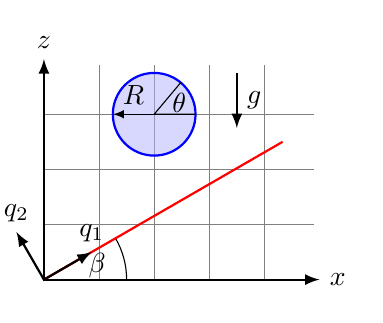
\begin{tikzpicture}[scale=0.7]
  \draw[style=help lines,step=1] (0,0) grid (4.9,3.9);
  \draw (0,0) -- (30:1.5) arc (30:0:1.5);
  \draw[latex-latex,thick] (0,4) node[above] {$z$} |- (5,0) node[right] {$x$};
  \draw[thick,draw=red] (0,0) -- (30:5);
  \draw (15:1) node {$\beta$};
  \begin{scope}[overlay,rotate=30]
    \draw[latex-latex,thick] (0,1) node[above] {$q_2$} |- (1,0) node[above] {$q_1$};
  \end{scope}
  \draw[fill=blue!30,draw=blue,fill opacity=0.5,thick] (2,3) circle (0.75);
  \begin{scope}[overlay,shift={(2,3)}]
    \draw (0.75,0) -- (0,0) -- (50:0.75);
    \draw (25:0.5) node {$\theta$};
    \draw[-latex] (0,0) -- (180:0.75) node[pos=0.5,above] {$R$};
  \end{scope}
  \draw[-latex,thick] (3.5,3.75) -- (3.5,2.75) node[pos=0.5,right] {$g$};
\end{tikzpicture}
\end{document}
